
%% bare_conf.tex
%% V1.3
%% 2007/01/11
%% by Michael Shell
%% See:
%% http://www.michaelshell.org/
%% for current contact information.
%%
%% This is a skeleton file demonstrating the use of IEEEtran.cls
%% (requires IEEEtran.cls version 1.7 or later) with an IEEE conference paper.
%%
%% Support sites:
%% http://www.michaelshell.org/tex/ieeetran/
%% http://www.ctan.org/tex-archive/macros/latex/contrib/IEEEtran/
%% and
%% http://www.ieee.org/

%%*************************************************************************
%% Legal Notice:
%% This code is offered as-is without any warranty either expressed or
%% implied; without even the implied warranty of MERCHANTABILITY or
%% FITNESS FOR A PARTICULAR PURPOSE!
%% User assumes all risk.
%% In no event shall IEEE or any contributor to this code be liable for
%% any damages or losses, including, but not limited to, incidental,
%% consequential, or any other damages, resulting from the use or misuse
%% of any information contained here.
%%
%% All comments are the opinions of their respective authors and are not
%% necessarily endorsed by the IEEE.
%%
%% This work is distributed under the LaTeX Project Public License (LPPL)
%% ( http://www.latex-project.org/ ) version 1.3, and may be freely used,
%% distributed and modified. A copy of the LPPL, version 1.3, is included
%% in the base LaTeX documentation of all distributions of LaTeX released
%% 2003/12/01 or later.
%% Retain all contribution notices and credits.
%% ** Modified files should be clearly indicated as such, including  **
%% ** renaming them and changing author support contact information. **
%%
%% File list of work: IEEEtran.cls, IEEEtran_HOWTO.pdf, bare_adv.tex,
%%                    bare_conf.tex, bare_jrnl.tex, bare_jrnl_compsoc.tex
%%*************************************************************************

% *** Authors should verify (and, if needed, correct) their LaTeX system  ***
% *** with the testflow diagnostic prior to trusting their LaTeX platform ***
% *** with production work. IEEE's font choices can trigger bugs that do  ***
% *** not appear when using other class files.                            ***
% The testflow support page is at:
% http://www.michaelshell.org/tex/testflow/



% Note that the a4paper option is mainly intended so that authors in
% countries using A4 can easily print to A4 and see how their papers will
% look in print - the typesetting of the document will not typically be
% affected with changes in paper size (but the bottom and side margins will).
% Use the testflow package mentioned above to verify correct handling of
% both paper sizes by the user's LaTeX system.
%
% Also note that the "draftcls" or "draftclsnofoot", not "draft", option
% should be used if it is desired that the figures are to be displayed in
% draft mode.
%
\documentclass[conference]{IEEEtran}
% Add the compsoc option for Computer Society conferences.
%
% If IEEEtran.cls has not been installed into the LaTeX system files,
% manually specify the path to it like:
% \documentclass[conference]{../sty/IEEEtran}





% Some very useful LaTeX packages include:
% (uncomment the ones you want to load)


% *** MISC UTILITY PACKAGES ***
%
%\usepackage{ifpdf}
% Heiko Oberdiek's ifpdf.sty is very useful if you need conditional
% compilation based on whether the output is pdf or dvi.
% usage:
% \ifpdf
%   % pdf code
% \else
%   % dvi code
% \fi
% The latest version of ifpdf.sty can be obtained from:
% http://www.ctan.org/tex-archive/macros/latex/contrib/oberdiek/
% Also, note that IEEEtran.cls V1.7 and later provides a builtin
% \ifCLASSINFOpdf conditional that works the same way.
% When switching from latex to pdflatex and vice-versa, the compiler may
% have to be run twice to clear warning/error messages.






% *** CITATION PACKAGES ***
%
%\usepackage{cite}
% cite.sty was written by Donald Arseneau
% V1.6 and later of IEEEtran pre-defines the format of the cite.sty package
% \cite{} output to follow that of IEEE. Loading the cite package will
% result in citation numbers being automatically sorted and properly
% "compressed/ranged". e.g., [1], [9], [2], [7], [5], [6] without using
% cite.sty will become [1], [2], [5]--[7], [9] using cite.sty. cite.sty's
% \cite will automatically add leading space, if needed. Use cite.sty's
% noadjust option (cite.sty V3.8 and later) if you want to turn this off.
% cite.sty is already installed on most LaTeX systems. Be sure and use
% version 4.0 (2003-05-27) and later if using hyperref.sty. cite.sty does
% not currently provide for hyperlinked citations.
% The latest version can be obtained at:
% http://www.ctan.org/tex-archive/macros/latex/contrib/cite/
% The documentation is contained in the cite.sty file itself.






% *** GRAPHICS RELATED PACKAGES ***
%
\ifCLASSINFOpdf
  % \usepackage[pdftex]{graphicx}
  % declare the path(s) where your graphic files are
  % \graphicspath{{../pdf/}{../jpeg/}}
  % and their extensions so you won't have to specify these with
  % every instance of \includegraphics
  % \DeclareGraphicsExtensions{.pdf,.jpeg,.png}
\else
  % or other class option (dvipsone, dvipdf, if not using dvips). graphicx
  % will default to the driver specified in the system graphics.cfg if no
  % driver is specified.
  % \usepackage[dvips]{graphicx}
  % declare the path(s) where your graphic files are
  % \graphicspath{{../eps/}}
  % and their extensions so you won't have to specify these with
  % every instance of \includegraphics
  % \DeclareGraphicsExtensions{.eps}
\fi
% graphicx was written by David Carlisle and Sebastian Rahtz. It is
% required if you want graphics, photos, etc. graphicx.sty is already
% installed on most LaTeX systems. The latest version and documentation can
% be obtained at:
% http://www.ctan.org/tex-archive/macros/latex/required/graphics/
% Another good source of documentation is "Using Imported Graphics in
% LaTeX2e" by Keith Reckdahl which can be found as epslatex.ps or
% epslatex.pdf at: http://www.ctan.org/tex-archive/info/
%
% latex, and pdflatex in dvi mode, support graphics in encapsulated
% postscript (.eps) format. pdflatex in pdf mode supports graphics
% in .pdf, .jpeg, .png and .mps (metapost) formats. Users should ensure
% that all non-photo figures use a vector format (.eps, .pdf, .mps) and
% not a bitmapped formats (.jpeg, .png). IEEE frowns on bitmapped formats
% which can result in "jaggedy"/blurry rendering of lines and letters as
% well as large increases in file sizes.
%
% You can find documentation about the pdfTeX application at:
% http://www.tug.org/applications/pdftex





% *** MATH PACKAGES ***
%
%\usepackage[cmex10]{amsmath}
% A popular package from the American Mathematical Society that provides
% many useful and powerful commands for dealing with mathematics. If using
% it, be sure to load this package with the cmex10 option to ensure that
% only type 1 fonts will utilized at all point sizes. Without this option,
% it is possible that some math symbols, particularly those within
% footnotes, will be rendered in bitmap form which will result in a
% document that can not be IEEE Xplore compliant!
%
% Also, note that the amsmath package sets \interdisplaylinepenalty to 10000
% thus preventing page breaks from occurring within multiline equations. Use:
%\interdisplaylinepenalty=2500
% after loading amsmath to restore such page breaks as IEEEtran.cls normally
% does. amsmath.sty is already installed on most LaTeX systems. The latest
% version and documentation can be obtained at:
% http://www.ctan.org/tex-archive/macros/latex/required/amslatex/math/





% *** SPECIALIZED LIST PACKAGES ***
%
%\usepackage{algorithmic}
% algorithmic.sty was written by Peter Williams and Rogerio Brito.
% This package provides an algorithmic environment fo describing algorithms.
% You can use the algorithmic environment in-text or within a figure
% environment to provide for a floating algorithm. Do NOT use the algorithm
% floating environment provided by algorithm.sty (by the same authors) or
% algorithm2e.sty (by Christophe Fiorio) as IEEE does not use dedicated
% algorithm float types and packages that provide these will not provide
% correct IEEE style captions. The latest version and documentation of
% algorithmic.sty can be obtained at:
% http://www.ctan.org/tex-archive/macros/latex/contrib/algorithms/
% There is also a support site at:
% http://algorithms.berlios.de/index.html
% Also of interest may be the (relatively newer and more customizable)
% algorithmicx.sty package by Szasz Janos:
% http://www.ctan.org/tex-archive/macros/latex/contrib/algorithmicx/




% *** ALIGNMENT PACKAGES ***
%
%\usepackage{array}
% Frank Mittelbach's and David Carlisle's array.sty patches and improves
% the standard LaTeX2e array and tabular environments to provide better
% appearance and additional user controls. As the default LaTeX2e table
% generation code is lacking to the point of almost being broken with
% respect to the quality of the end results, all users are strongly
% advised to use an enhanced (at the very least that provided by array.sty)
% set of table tools. array.sty is already installed on most systems. The
% latest version and documentation can be obtained at:
% http://www.ctan.org/tex-archive/macros/latex/required/tools/


%\usepackage{mdwmath}
%\usepackage{mdwtab}
% Also highly recommended is Mark Wooding's extremely powerful MDW tools,
% especially mdwmath.sty and mdwtab.sty which are used to format equations
% and tables, respectively. The MDWtools set is already installed on most
% LaTeX systems. The lastest version and documentation is available at:
% http://www.ctan.org/tex-archive/macros/latex/contrib/mdwtools/


% IEEEtran contains the IEEEeqnarray family of commands that can be used to
% generate multiline equations as well as matrices, tables, etc., of high
% quality.


%\usepackage{eqparbox}
% Also of notable interest is Scott Pakin's eqparbox package for creating
% (automatically sized) equal width boxes - aka "natural width parboxes".
% Available at:
% http://www.ctan.org/tex-archive/macros/latex/contrib/eqparbox/





% *** SUBFIGURE PACKAGES ***
%\usepackage[tight,footnotesize]{subfigure}
% subfigure.sty was written by Steven Douglas Cochran. This package makes it
% easy to put subfigures in your figures. e.g., "Figure 1a and 1b". For IEEE
% work, it is a good idea to load it with the tight package option to reduce
% the amount of white space around the subfigures. subfigure.sty is already
% installed on most LaTeX systems. The latest version and documentation can
% be obtained at:
% http://www.ctan.org/tex-archive/obsolete/macros/latex/contrib/subfigure/
% subfigure.sty has been superceeded by subfig.sty.



%\usepackage[caption=false]{caption}
%\usepackage[font=footnotesize]{subfig}
% subfig.sty, also written by Steven Douglas Cochran, is the modern
% replacement for subfigure.sty. However, subfig.sty requires and
% automatically loads Axel Sommerfeldt's caption.sty which will override
% IEEEtran.cls handling of captions and this will result in nonIEEE style
% figure/table captions. To prevent this problem, be sure and preload
% caption.sty with its "caption=false" package option. This is will preserve
% IEEEtran.cls handing of captions. Version 1.3 (2005/06/28) and later
% (recommended due to many improvements over 1.2) of subfig.sty supports
% the caption=false option directly:
%\usepackage[caption=false,font=footnotesize]{subfig}
%
% The latest version and documentation can be obtained at:
% http://www.ctan.org/tex-archive/macros/latex/contrib/subfig/
% The latest version and documentation of caption.sty can be obtained at:
% http://www.ctan.org/tex-archive/macros/latex/contrib/caption/




% *** FLOAT PACKAGES ***
%
%\usepackage{fixltx2e}
% fixltx2e, the successor to the earlier fix2col.sty, was written by
% Frank Mittelbach and David Carlisle. This package corrects a few problems
% in the LaTeX2e kernel, the most notable of which is that in current
% LaTeX2e releases, the ordering of single and double column floats is not
% guaranteed to be preserved. Thus, an unpatched LaTeX2e can allow a
% single column figure to be placed prior to an earlier double column
% figure. The latest version and documentation can be found at:
% http://www.ctan.org/tex-archive/macros/latex/base/



%\usepackage{stfloats}
% stfloats.sty was written by Sigitas Tolusis. This package gives LaTeX2e
% the ability to do double column floats at the bottom of the page as well
% as the top. (e.g., "\begin{figure*}[!b]" is not normally possible in
% LaTeX2e). It also provides a command:
%\fnbelowfloat
% to enable the placement of footnotes below bottom floats (the standard
% LaTeX2e kernel puts them above bottom floats). This is an invasive package
% which rewrites many portions of the LaTeX2e float routines. It may not work
% with other packages that modify the LaTeX2e float routines. The latest
% version and documentation can be obtained at:
% http://www.ctan.org/tex-archive/macros/latex/contrib/sttools/
% Documentation is contained in the stfloats.sty comments as well as in the
% presfull.pdf file. Do not use the stfloats baselinefloat ability as IEEE
% does not allow \baselineskip to stretch. Authors submitting work to the
% IEEE should note that IEEE rarely uses double column equations and
% that authors should try to avoid such use. Do not be tempted to use the
% cuted.sty or midfloat.sty packages (also by Sigitas Tolusis) as IEEE does
% not format its papers in such ways.





% *** PDF, URL AND HYPERLINK PACKAGES ***
%
%\usepackage{url}
% url.sty was written by Donald Arseneau. It provides better support for
% handling and breaking URLs. url.sty is already installed on most LaTeX
% systems. The latest version can be obtained at:
% http://www.ctan.org/tex-archive/macros/latex/contrib/misc/
% Read the url.sty source comments for usage information. Basically,
% \url{my_url_here}.





% *** Do not adjust lengths that control margins, column widths, etc. ***
% *** Do not use packages that alter fonts (such as pslatex).         ***
% There should be no need to do such things with IEEEtran.cls V1.6 and later.
% (Unless specifically asked to do so by the journal or conference you plan
% to submit to, of course. )


% correct bad hyphenation here
\hyphenation{op-tical net-works semi-conduc-tor}

\usepackage{algpseudocode}
\usepackage{algorithm}
\usepackage{subfig}
\usepackage{amsthm}
\usepackage{graphicx}
\usepackage{multirow}
\theoremstyle{definition}
\newtheorem{definition}{Definition}
\newtheorem*{theorem}{Theorem}

\renewcommand{\algorithmicrequire}{ \textbf{Input:}} \renewcommand{\algorithmicensure}{ \textbf{Output:}}
\floatname{algorithm}{Strategy}


\begin{document}
%
% paper title
% can use linebreaks \\ within to get better formatting as desired
\title{Top-down and Bottom-up Strategies for Generating Incremental Covering Arrays}


% author names and affiliations
% use a multiple column layout for up to three different
% affiliations
%\author{\IEEEauthorblockN{Xintao Niu and Changhai nie}
%\IEEEauthorblockA{State Key Laboratory for Novel \\
%Software Technology\\
%Nanjing University, China, 210023\\
%Email: niuxintao@gmail.com}
%\and
%\IEEEauthorblockN{Changhai nie}
%\IEEEauthorblockA{State Key Laboratory for Novel \\
%Software Technology\\
%Nanjing University, China, 210023\\
%Email: changhainie@nju.edu.com}
%\and
%\IEEEauthorblockN{Hareton Leung}
%\IEEEauthorblockA{Department of computing \\
%Hong Kong Polytechnic University\\
%Kowloon, Hong Kong\\
%Email: cshleung@comp.polyu.edu.hk}
%\and
%\IEEEauthorblockN{Jeff Y. Lei}
%\IEEEauthorblockA{Department of Computer Science\\
%and Engineering\\
%The University of Texas at Arlington\\
%Email: ylei@cse.uta.edu}
%\and
%\IEEEauthorblockN{Xiaoyin Wang}
%\IEEEauthorblockA{
%        Department of Computer Science \\
%        University of Texas at San Antonio\\
% %      \affaddr{China, 211171}\\
%%       \email{xujiaxi@njxzc.edu.cn} \\
%       Email: Xiaoyin.Wang@utsa.edu}
%}
% conference papers do not typically use \thanks and this command
% is locked out in conference mode. If really needed, such as for
% the acknowledgment of grants, issue a \IEEEoverridecommandlockouts
% after \documentclass

% for over three affiliations, or if they all won't fit within the width
% of the page, use this alternative format:
%
\author{\IEEEauthorblockN{Xintao Niu\IEEEauthorrefmark{1},
Changhai Nie\IEEEauthorrefmark{1},
Hareton Leung\IEEEauthorrefmark{2},
Jeff Y. Lei\IEEEauthorrefmark{3},
Xiaoyin Wang\IEEEauthorrefmark{4},
Yan Wang \IEEEauthorrefmark{5},
Mengfan Zeng\IEEEauthorrefmark{1}, and
Jiaxi Xu \IEEEauthorrefmark{5}}
\IEEEauthorblockA{\IEEEauthorrefmark{1}State Key Laboratory for Novel Software Technology\\
Nanjing University, China, 210023\\
Email: niuxintao@gmail.com, changhainie@nju.edu.cn, zengmengfan@foxmail.com}
\IEEEauthorblockA{\IEEEauthorrefmark{2}Department of Computing Hong Kong Polytechnic University\\
Kowloon, Hong Kong\\
Email: cshleung@comp.polyu.edu.hk}
\IEEEauthorblockA{\IEEEauthorrefmark{3} Dpartment of Computer Science and Engineering\\
The University of Texas at Arlington\\
Email: ylei@cse.uta.edu}
\IEEEauthorblockA{\IEEEauthorrefmark{4} Department of Computer Science \\
University of Texas at San Antonio\\
Email: Xiaoyin.Wang@utsa.edu}
\IEEEauthorblockA{\IEEEauthorrefmark{5} School of Information Engineering\\
Nanjing Xiaozhuang University\\
Email: wangyan@njxzc.edu.cn, xujiaxi@njxzc.edu.cn}
}




% use for special paper notices
%\IEEEspecialpapernotice{(Invited Paper)}




% make the title area
\maketitle


\begin{abstract}
%\boldmath
Combinatorial Testing (CT) is an effective technique for testing the interactions of factors in the Software Under Test (SUT). By designing an efficient set of test cases, i.e., a covering array, CT aims to check every possible valid interaction in SUT. Most existing covering array generation algorithms require a given \emph{degree} \emph{t} in prior, such that only the interactions with no more than $t$ factors are to be checked.  In practice, however, the value of $t$ cannot be properly determined, especially for systems with complex interaction space.  Hence, incremental covering arrays are preferred. In this paper, we propose two strategies for generating incremental covering arrays which can increase the coverage strength when required. A preliminary evaluation of the two strategies is presented, which shows that both strategies have their own advantages with respect to covering array size.
\end{abstract}
% IEEEtran.cls defaults to using nonbold math in the Abstract.
% This preserves the distinction between vectors and scalars. However,
% if the conference you are submitting to favors bold math in the abstract,
% then you can use LaTeX's standard command \boldmath at the very start
% of the abstract to achieve this. Many IEEE journals/conferences frown on
% math in the abstract anyway.

% no keywords

%\category{D.2.5}{Software Engineering}{Testing and debugging}[Debugging aids,testing tools]
%
%\terms{Reliability, Verification}
\begin{IEEEkeywords}
Combinatorial Testing, Covering Array, Incremental Covering Array, Bottom-up and Top-down strategy
\end{IEEEkeywords}
%\IEEEkeywords{
%  }
%\keywords{


% For peer review papers, you can put extra information on the cover
% page as needed:
% \ifCLASSOPTIONpeerreview
% \begin{center} \bfseries EDICS Category: 3-BBND \end{center}
% \fi
%
% For peerreview papers, this IEEEtran command inserts a page break and
% creates the second title. It will be ignored for other modes.
\IEEEpeerreviewmaketitle



\section{Introduction}
With the growing complexity and scale of modern software systems, various factors, such as input values and configure options, can affect the behaviour of a system. Even worse, some interactions between them can trigger unexpected negative effects on the software. To ensure the correctness and quality of the software system, it is desirable to detect and locate these \emph{bad} interactions. The simplest way to solve this problem is to perform exhaustive testing for all the possible valid interactions of the system. It is, however, not practical due to the combinatorial explosion. Therefore, the selection of a group of representative test cases from the whole testing space is required.

Combinatorial testing has been proven to be effective in sampling an effective set of test cases\cite{nie2011survey}. It works by generating a relatively small set of test cases, i.e., a covering array, to test the interactions involving a given number of factors that may affect the behavior of a system. The number of factors involved in those selected interactions is limited in a moderate range, which is usually from 2 to 6 \cite{kuhn2002investigation}.

% The justification behind of this range is that based on empirical studies \cite{kuhn2002investigation}, most failures in the system are caused by the interactions with number of involved factors no more than 6 \cite{kuhn2002investigation}. And hence can fulfil testing requirement at most time.

Many algorithms have been proposed to generate covering arrays. Despite many differences between them,  those works all assume that the degree \emph{t} is a given priori.  The degree \emph{t} indicates the largest number of factors involved in the interactions to be covered, and the corresponding covering arrays which can satisfy this coverage criteria is called \emph{t}-way covering arrays. In practice, however, the value of \emph{t} is difficult to determine due to two reasons as follows. First, many software systems suffer from complex interaction space which make it challenging to estimate \emph{t}. In such case, even experienced testers can make mistakes and estimate a wrong value for \emph{t}, which can significantly affect the effectiveness and efficiency of CT. Specifically, if $t$ is estimated to be larger than required, many redundant test cases will be generated, which is a waste of computing resource. And if $t$ is estimated to be smaller than required, then the generated covering array is not sufficient to obtain an effective test set. Second, even though \emph{t} has been properly determined, there may not be enough time to completely execute all the test cases in the covering array. This is because testing software only makes sense before the next version is released. This time interval between two release versions may sometimes be too short for a complete testing of a high-strength covering array, especially in the scenario of continuous integration \cite{fouche2009incremental}.

%In fact, in the worst case, any interaction with any strength can have an distinct affect of the SUT.

To address these shortcomings of traditional covering arrays, the notion of incremental covering array \cite{fouche2009incremental} has been proposed. Such object can be deemed as adaptive covering array, which can increase the degree \emph{t} when required. As it can generate higher strength covering array based on lower strength covering array, it can reduce the cost when comparing with generating multiple ways of covering arrays. Additionally, it can be better applied on testing the software of which the released time is  frequently changed and cannot be predicted. Another advantage for generating incremental covering array is that, testers can detect most faults in the software as soon as possible. This is because according to \cite{kuhn2002investigation}, most faults (about 70\% to 80\%) are caused by 2-degree interactions, and almost all faults can be covered by 6-way covering arrays. As incremental covering arrays first cover those lower-degree interactions, the faults caused by them will be detected sooner.

% the incremental covering array is a merged covering array for multiple covering arrays.

In consideration of the size of the total number of test cases, we argue that this approach of generating incremental covering array may produce too many test cases. This is obvious, as generating higher-strength covering array based on the lower-strength covering array (called \emph{bottom-up} strategy later) does not aim to optimize the size of the higher-strength covering array. As a result, it may generate more test cases than those approaches that focus on generating a particular higher-strength covering array.

Then, a natural question, and also the motivation of this paper is, \textbf{is it possible to generate an incremental covering array with the same number of the overall test cases as those by the particular high-way covering array generation algorithms ?}  Due to the obvious conclusion that any high way covering array must cover all the lower way interactions, the answer for this question is \emph{yes}, as we can just apply a particular covering array generation algorithm to generate the high-strength covering array, and then generate the lower-strength covering arrays by extracting some subset of the test cases which can cover all the lower degree interactions. We refer to this strategy as the \emph{top-down} strategy.

In this paper, we propose these two strategies and evaluate their performance by comparing them at constructing several incremental covering arrays. The results of the experiments showed that the \emph{top-down} strategy has an significant advantage at the size of the higher-strength covering array, while the \emph{bottom-up} strategy is better at constructing those lower-strength covering arrays with smaller size. Based on this observation, we applied our two strategies on testing an industrial software (Tomcat). The results of this empirical study showed that our approach generates smaller size of test cases than traditional approach, while keeps a high rate of fault detection.

%The answer is yes.
%For this, And also the key idea of this paper : To generate higher strength covering array from the lower strength, may be not effective at the size of the overall needed test cases. This can be easily understood, as it is not focus on the  higher covering array, which should . to in the .
%
%Then a . In fact, to execute the test cases , not mean to generate them in the order.


% no \IEEEPARstart
%Modern software are becoming more and more complicated. Combinatorial testing, as a black, has been proven to be effecive.
%
%
%and hence makes applying CT a challenge task.
%
%
%In the other hand, simply generated different covering arrays will be , as many test cases in the covering array may be redundant.
Our contributions include:

 \begin{enumerate}
 \item  We propose a formal description of incremental covering array, and give a proof of the existence of it.
 \item  We propose two strategies for generating incremental covering arrays.
 \item  We conduct a series of experiments to evaluate the characteristics of these two strategies, and compare the performance of our approach with traditional approach.
 %\item  We apply our approach on testing an industrial software and compare the performance between the traditional approach with ours.
 \item  We offer a guideline for selecting which strategy when generating incremental covering array in practice.
\end{enumerate}
%\section{Motivation}
%

\section{Background}
This section gives some formal definitions related to CT. Assume that the behaviour of SUT is influenced by \emph{k} parameters, and each parameter $p_{i}$ has $a_{i}$ discrete values from the finite set $V_{i}$, i.e., $a_{i}$ = $|V_{i}|$ ($i$ = 1,2,..k). Then a \emph{test case} of the SUT is a group of values that are assigned to each parameter, which can be denoted as ($v_{1}, v_{2}, ..., v_{k}$). An $t$-degree interaction can be formally denoted as $(-, ..., v_{n_{1}}, -, ..., v_{n_{2}},-, ...,v_{n_{t}}, -, ...)$, where some t parameters have fixed values and other irrelevant parameters are represented as "-". In fact, a test case can be regarded as a $k$-degree interaction.


\subsection{Covering array}

\begin{definition}A $t$-way \emph{covering array} $MCA(N; t, k,$ $(a_{1}, a_{2}, ..., a_{k})$) is a test set in the form of $N \times k$ table, where each row represents a \emph{test case} and each column represents a parameter.  For any \emph{t} columns, each possible \emph{t}-degree interaction of the $t$ parameters must appear at least once. When $ a_{1} = a_{2} = ... = a_{k} = v $, a $t$-way covering array can be denoted as $CA(N; t, k, v)$.
\end{definition}


For example, Table \ref{ica_example} (a) shows a 2-way covering array $CA(5;2,4,2)$ for the SUT with 4 boolean parameters. For any two columns, any 2-degree interaction is covered.  Covering array has proven to be effective in detecting the failures caused by interactions of parameters of the SUT. Many existing algorithms focus on constructing covering arrays such that the number of test cases, i.e., $N$, can be as small as possible.


\subsection{Incremental covering array}

\begin{definition}
An incremental covering array $ICA([N_{t_{1}},$ $N_{t_{1} + 1},...,N_{t_{2}}];[t_{1},t_{2}]$ $, k, (a_{1},a_{2},...,a_{k}))$ is a test set in the form of $N_{t_{2}} \times k$ table, where $t_{1} < t_{2}$ and  $N_{t_{1}}<N_{t_{1} + 1} <$ $,...,$ $< N_{t_{2}}$.  In this table, the first $N_{t_{i}}$ lines ($t_{1}\leq t_{i} \leq t_{2}$) is a covering array $MCA(N_{t_{i}}; t_{1} + i, k , (a_{1},a_{2},...,a_{k}))$.

 When $ a_{1} = a_{2} = ... = a_{k} = v $, an incremental covering array can be denoted as $ICA([N_{t_{1}},$ $N_{t_{1} + 1},...,N_{t_{2}}];[t_{1},t_{2}], k,$ $ v)$.
\end{definition}


Table \ref{ica_example} shows an example of incremental covering array, in which the two-way covering array $CA(5;2,4,2)$ is a subset of the three-way covering array $CA(9;3,4,2)$, which is also an incremental covering array $ICA([5,9];[2,3],4,2)$.

\begin{table}[htbp]
  \small
  \centering
  \caption{Experiment of Incremental covering array}
  \label{ica_example}

    \begin{tabular}{c}
 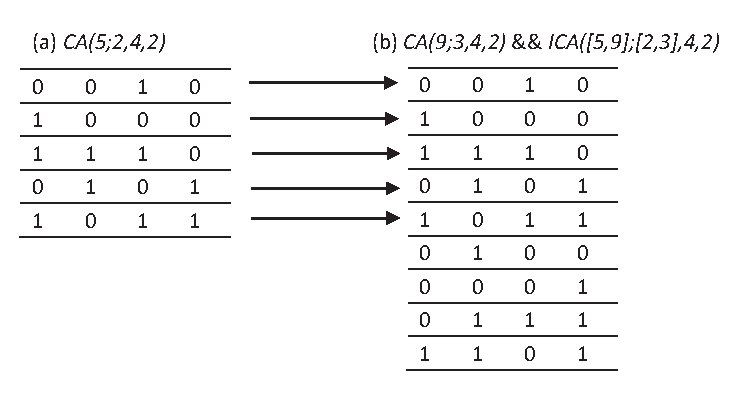
\includegraphics[width=3.4in]{incremental_covering_ex.eps}
    \end{tabular}%

\end{table}

%\begin{table}[htbp]
%  \small
%  \centering
%  \caption{Experiment of Incremental covering array}
%  \label{ica_example}
%  \subfloat[$CA(5;2,4,2)$]{%
%    \hspace{.5cm}%
%    \begin{tabular}{c c c c}
%        \hline
%
%        0 & 0 & 1 & 0 \\  \hline
%        1 & 0 & 0 & 0 \\ \hline
%        1 & 1 & 1 & 0 \\ \hline
%        0 & 1 & 0 & 1 \\ \hline
%        1 & 0 & 1 & 1 \\ \hline
%
%        \hline
%    \end{tabular}%
%    \hspace{.5cm}%
%  }\hspace{1cm}
%  \subfloat[$CA(9;3,4,2)$]{%
%    \hspace{.5cm}%
%    \begin{tabular}{c c c c}
%        \hline
%
%        0 & 0 & 1 & 0 \\  \hline
%        1 & 0 & 0 & 0 \\ \hline
%        1 & 1 & 1 & 0 \\ \hline
%        0 & 1 & 0 & 1 \\ \hline
%        1 & 0 & 1 & 1 \\ \hline
%        0 & 1 & 0 & 0 \\ \hline
%        0 & 0 & 0 & 1 \\ \hline
%        0 & 1 & 1 & 1 \\ \hline
%        1 & 1 & 0 & 1 \\ \hline
%
%    \end{tabular}%
%    \hspace{.5cm}%
%  }
%\end{table}


\begin{theorem}
%Each $ICA([N_{t_{1}},N_{t_{1} + 1},...,N_{t_{2}}];[t_{1},t_{2}]$ $, k, v)$ is a $CA(N_{t_{2}}; t_{2}, k, v)$ covering array.
For each covering array $MCA(N_{t_{2}}; t_{2}, k, (a_{1},a_{2},$ $...,a_{k}))$, we can find an $ICA([N_{t_{1}},N_{t_{1} + 1},...,N_{t_{2}}];[t_{1},t_{2}]$ $, k, (a_{1},a_{2},$ $...,a_{k}))$, s.t., their test cases are the same.
\end{theorem}

\begin{proof}
%According to the definition of $ICA$, it can be easily got that $ICA([N_{t_{1}},N_{t_{1} + 1},...,N_{t_{2}}];[t_{1},t_{2}]$ $, k, v)$ is a $CA(N_{t_{2}}; t_{2}, k, v)$ covering array. For the second statement,
We just need to prove that for any covering array, $MCA(N_{t}; t, k, (a_{1},a_{2},$ $...,a_{k}))$, we can find a $MCA(N_{t-1}; t-1, k, (a_{1},a_{2},$ $...,a_{k}))$, such that, $N_{t-1} < N_{t}$ and for any test case  $f \in MCA(N_{t-1}; t-1, k, (a_{1},a_{2},$ $...,a_{k}))$, it has $f \in MCA(N_{t}; t, k, (a_{1},a_{2},$ $...,a_{k}))$.

 First, $MCA(N_{t}; t, k, (a_{1},a_{2},$ $...,a_{k}))$ itself must be an $MCA(N_{t}; t - 1, k, (a_{1},a_{2},$ $...,a_{k}))$, as it must cover all the $(t$ $ -1)$-degree interactions.

 Then, assume to obtain a $(t-1)$-way covering array, any one test case in $MCA(N_{t}; t, k, (a_{1},a_{2},$ $...,a_{k}))$ can not be reduced. With this assumption, any test case will cover at least one $(t-1)$-degree interaction that only appears in this test case. Without loss of generality,  let test case  ($v_{1}, v_{2}, ..., v_{k}$) cover the $(t-1)$-degree interaction $(-, ..., v_{p_{1}},...-,... v_{p_{2}},...,-, ..., v_{p_{t-1}},...-...,v_{p_{t}},...,-, ...)$ which only appears in the test case. Then obviously the $t$-degree interaction $(v_{1}', ..., v_{p_{1}},...-,... v_{p_{2}},...,-, ..., v_{p_{t-1}},...-...,v_{p_{t}},...,-, ...)$  ($v_{1}' \neq v_{1}$) will never be covered by any test case in $MCA(N_{t}; t, k, (a_{1},a_{2},$ $...,a_{k}))$, and hence $MCA(N_{t}; t, k, (a_{1},a_{2},$ $...,a_{k}))$ is not a $t$-way covering array (Note this is based on that the parameter can take on more than one value).

 This is a contradiction, and means that we can reduce at least one test case in $MCA(N_{t}; t, k, (a_{1},a_{2},$ $...,a_{k}))$, so that it is still a $(t-1)$-way covering array.
\end{proof}

This theorem shows the existence of the incremental covering arrays. As discussed before, generating the incremental covering arrays is of importance, as it supports adaptively increasing the coverage strength. According to this theorem, when testing a SUT, testers can firstly execute the lowest-strength covering array in the incremental covering arrays, and then execute additional test cases from those higher-strength covering arrays as required. The reuse of previously executed test cases will reduce the cost for generating multiple different-ways covering arrays.

\section{Generating incremental covering arrays}
This section presents two strategies to generate the incremental covering arrays. The first strategy, i.e., the \emph{bottom-up} strategy starts from generating the lowest-strength covering array and then the higher-strength ones. The second strategy, i.e., the  \emph{top-down} strategy firstly generated the highest-strength covering array, then the lower-strength covering array.

\subsection{Bottom-up strategy}
This strategy is listed as Strategy 1.
\begin{algorithm}
  \caption{Bottom-up strategy}
  \begin{algorithmic}[1]
     \Require
     $Params$ \Comment{Parameters (and their values)}

     $t_{1}$ \Comment{the lowest strength}
     %$s_{fixed}$ \Comment{fixed part}

     $t_{2}$ \Comment{the highest strength}

     \Ensure  $ICA$ \Comment{the incremental covering arrays}

    % \While{\textbf{not} $t_{uncovered}$ is not empty}
      \State $ICA \leftarrow Empty Set$
       \For {$t_{i} = t_{1};\ t_{i} \leq  t_{2};\ t_{i}\ ++$}
         \State $CA_{i} \leftarrow  Empty Set $
         \If {$t_{i} == t_{1}$}
                \State $CA_{i} \leftarrow CA\_Gen(Params, t_{i})$
         \Else
             \State $CA_{i} \leftarrow extend(Params, t_{i}, CA_{i - 1})$
        \EndIf

        \State $ICA.append(CA_{i})$
      \EndFor

     \State \Return $ICA$
  \end{algorithmic}
\end{algorithm}
The inputs for this strategy consists of the values for each parameter of the SUT --$Params$,  the lowest strength $t_{1}$ of the covering array in the incremental covering array, and the highest strength $t_{2}$ of the covering array . The output of this strategy is an incremental covering array -- $ICA$.

This strategy generates the covering array from lower-strength to higher-strength (line 2). If the current coverage strength $t_{i}$ is equal to $t_{1}$, it just utilizes a covering array generation algorithm to generate the particular covering array (line 4 - 5). Otherwise, it will first take the previous generated covering array $CA_{i - 1}$ as seeds, and then utilize covering array generation algorithm to append additional test cases to satisfy higher coverage criteria (line 6 - 7).
%the example for . Consider we are testing a object, initially, we believe 1 way is enough, but when we give so, it find that is not , then we must increase the , to three way. In such a case, to take a Coverin array to regenerate 3-way covering array is follish, as it may introuduce many redunenta.t For example, many 3 way schemas in fact have been checked before.
%
%Then it is of course we need to generate the coverin array based on the previous covering array, such that we can utilze the previous tesing results. For this, a natural idea, is to set the as the seeds, like this.

Fig.\ref{increase-example} presents an example for constructing $ICA([6,13,24];$ $  [2,4], 5, 2)$ by this strategy. In this example, the covering array generation algorithm used is AETG \cite{cohen1997aetg}. The two-way covering array (test cases $c_{1}$ to $c_{6}$) is directly generated, and the three-way covering array (test cases $c_{1}$ to $ c_{13}$) is generated by adding additional test cases (test cases $c_{7}$ to $c_{13}$) based on the previous two-way covering array. The four-way covering array (test cases $c_{1}$ to $c_{24}$) is constructed on the previous three-way covering array. In total, to reach the 4-way covering array, 24 test cases are needed for this strategy.
\begin{figure}
\center
 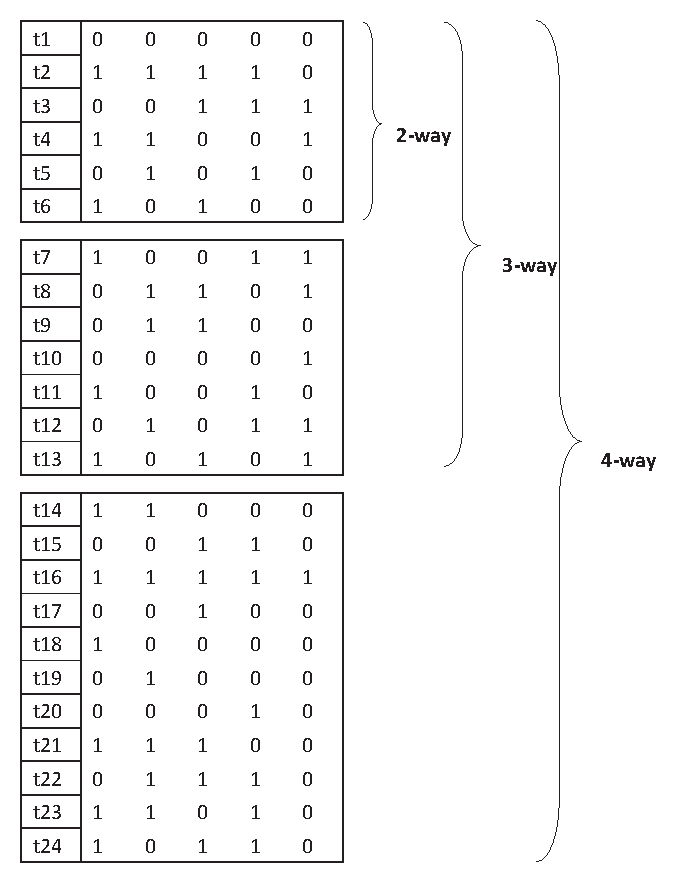
\includegraphics[width=3.0in]{increase_example.eps}
\caption{Bottom-up strategy example}
\label{increase-example}
\end{figure}

\subsection{Top-down strategy}
This strategy is listed as Strategy 2, which generates covering arrays in the opposite order (line 2) of the bottom-up strategy. Similarly, if the current coverage strength $t_{i}$ is equal to $t_{2}$, it directly generates the particular covering array (line 4 - 5). Otherwise, it will extract the covering array from a higher covering array ($CA_{i + 1}$) (line 6 - 7).



%Another reason we does not focus on obtaining the minimal size of $CA_{i}$, is that even though we have, it does not have so that $CA_{i - 1}$.

%Now let us think the following problem, as the . If we had first generate the 3-way covering array, and .
%
%need to . And hence then , we need to increase the degree, as . To . Then first, a natural
\begin{algorithm}
  \caption{Top-down strategy}
  \begin{algorithmic}[1]
    \Require
     $Params$ \Comment{Parameters (and their values)}

     $t_{1}$ \Comment{the lowest strength}
     %$s_{fixed}$ \Comment{fixed part}

     $t_{2}$ \Comment{the highest strength}

     \Ensure  $ICA$ \Comment{the incremental covering arrays}

    % \While{\textbf{not} $t_{uncovered}$ is not empty}
      \State $ICA \leftarrow Empty Set$
       \For {$t_{i} = t_{2};\ t_{i} \geq  t_{1};\ t_{i}\  -- $}
         \State $CA_{i} \leftarrow  Empty Set $
         \If {$t_{i} == t_{2}$}
                \State $CA_{i} \leftarrow CA\_Gen(Params, t_{i})$
         \Else
              \State $CA_{i} \leftarrow  extract(Params, t_{i}, CA_{i + 1})$
%             \While{$t_{i}$-way coverage is not satisfied}
%                \State $test \leftarrow selected(CA_{i + 1})$
%                \State $CA_{i}.append(test)$
%             \EndWhile
        \EndIf

        \State $ICA.append(CA_{i})$
      \EndFor

     \State \Return $ICA$
  \end{algorithmic}
\end{algorithm}

An example for this strategy is given in Fig.\ref{decrease-example}. In this example, we first generated the 4-way covering array $CA(16; 4, 5, 2)$. Then we selected 14 test cases to form a three-covering array $CA(14; 3, 5, 2)$. Next the two-way covering array $CA(8; 2, 5, 2)$ is extracted from $CA(14; 3, 5, 2)$. The rows with dark background from the higher-strength covering arrays represent those selected test cases.

\begin{figure}
 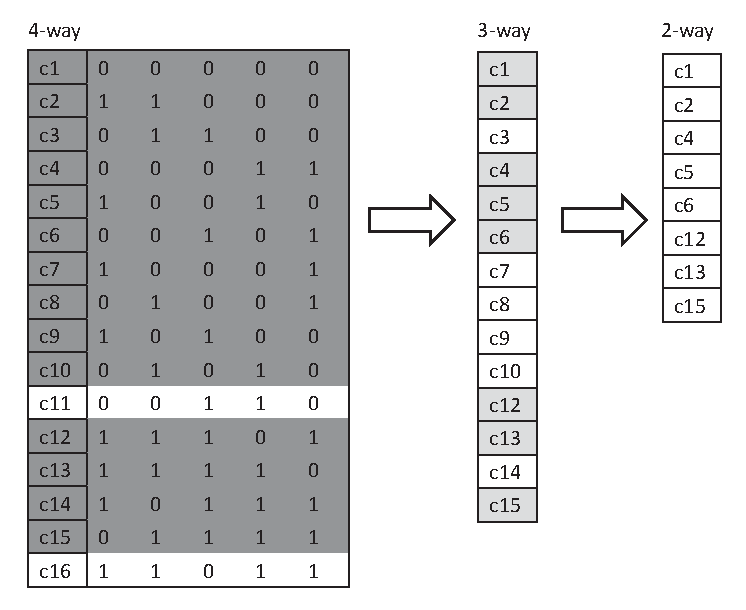
\includegraphics[width=3.4in]{decrease_example.eps}
\caption{Top-down strategy example}
\label{decrease-example}
\end{figure}


From the two examples, an obvious observation is that for the \emph{top-down} strategy, it has a significant advantage over the \emph{bottom-up} strategy with respect to the size of the 4-way covering array (16 for \emph{top-down} and 24 for \emph{bottom-up}). But when  considering the lower-strength covering arrays, the \emph{bottom-up} strategy performs better (13 and 6 for \emph{bottom-up}, while 14 and 8 for \emph{top-down} respectively).  To evaluate the generality of this observation , we conduct experiments in the next section.


%\section{}


\section{Implementation of the approach}
In this section, we will describe a specific implementation of the two strategies proposed in the previous section.

\subsection{Covering array generation method}
Our covering array generation approach is IPOG \cite{lei2007ipog,lei2008ipog,yu2013efficient}, which firstly builds a \emph{t}-way test set for the first \emph{t} parameters, then extends the test set to build a t-way test set for the first t+1 parameters, and then continues to extend the test set until it builds a t-way test set for all the parameters. We select this algorithm mainly because of its efficiency, that is, it can quickly generate a t-way covering array even though \emph{t} is a relatively large number (up to 6). This is important, as in our experiment section, some subjects contain an extremely large input space, which is unfavorable to apply some time-consuming covering array generation approaches.

\subsection{Constraints handling}
Our constraints handling technique is based on Minimum Forbidden Tuples (MFTs) \cite{yu2014combinatorial,yu2015constraint}, which is well supported by IPOG generation algorithm. A forbidden tuple is a tuple as the value assignment of some parameters that violates constraints. A minimum forbidden tuple is a forbidden tuple of minimum size that covers no other forbidden tuples. Given some constraints for one SUT, we should compute all the MFTs of the SUT, and then limit the test cases to the ones that do not contain any tuple in the MFTs.

\subsection{Seeding technique}
Seeding test cases is the key part for the bottom-up strategy, which regards the lower-way covering array as the seeds of the higher-way covering array. Specifically, we need to eliminated those higher-degree tuples that have already been covered by the lower-way covering array. Then we just need to continue the test case generation approach  to cover the remaining un-covered higher-degree tuples.


\subsection{Extract lower-way covering array}
This is the key part for the top-down strategy. The extraction process is a greedy approach in this paper. For any $t_{i+1}$ covering array, at each iteration, we only select the test case which can cover most uncovered $t_{i}$-degree interactions from the $t_{i+1}$-way covering array. The selection process repeats until we obtain a complete $t_{i}$-way covering array.  Note that this greedy selection does not promise to obtain the $CA_{i}$ covering array with the minimal size. But to get the minimal size, we need to exhaustively check every possible subset of the higher-covering array $CA_{i+1}$. This is impractical if the size of $CA_{i + 1}$ is too large.

\section{Experiments and Results}
\subsection{Research Questions}
We set up the following four research questions to investigate
the effectiveness and the efficiency of our approach.

RQ1. Compared with the traditional t-way test generation,
can DICOT deliver higher t0-way coverage with
higher interaction strength t0(> t)? If so, how big
are the improvement and computational overhead?

RQ2. Compared with the Enumerating Choice (EC) approach,
how eective and ecient is DICOT w. r. t.
t0(> t)-way coverage and computational overhead?

RQ3. Compared with the DT approach, how eective and
ecient is DICOT w. r. t. the t-way test suite size and
t0(> t)-way coverage?

RQ4. How different is the performance when using Hamming
distance and chi-square distance as a distance
metric in DICOT?DICOT employs another appr
This section describes the experiments.
\subsection{Benchmarks}
We used 55 SUT as the subjects of our experiments, which are shown in Table \ref{model_of_sut_of_subjects}. These subjects are wildly used to evaluate the performance of the covering array generation approach. Among these subjects, the first 20 subjects (from \emph{Banking1} to \emph{Telecom}), come from a recent benchmark created by Segall et al \cite{segall2011using}, which have already been used in several works \cite{jia2015learning,choi2016distance}. There 20 subjects cover a wide range of applications, including telecommunications, health care, storage and banking systems.  The following five subjects (from \emph{SPIN-S}  to \emph{Bugzilla} ) were firstly introduced by Cohen et al. \cite{cohen2007interaction,cohen2008constructing}. Among them, SPIN-S and SPIN-V are two components for model simulation and verification, GCC is a compiler system, Apache is a web server application, and Bugzilla is a web-based bug tracking system. These five subjects have been wildly used in literatures \cite{kuhn2006pseudo,cohen2007interaction,cohen2008constructing,garvin2009improved,garvin2011evaluating,lin2015tca,choi2016distance}. The last 30 (from Syn1 to Syn30) are synthetic subject models that are generated by Cohen et al. \cite{cohen2008constructing}. These synthetic subject models are designed with similar characterization (input space, constraints, etc.) with those real subjects and have been used in following studies\cite{garvin2009improved,garvin2011evaluating,lin2015tca,choi2016distance}.

In Table \ref{model_of_sut_of_subjects}, the model is presented in the abbreviated form $\#values^{\#number\ of\ parameters}$, e.g., $7^{3}6^{2}$ indicates the software has 3 parameters that can take 7 values and 2 parameters take 6 values.  The constraint is presented in the form $\#degree^{\#number\ of\ constraints}$, e.g., $2^{3}3^{18}$ means that the SUT contains 3 constraints with  2-degree and 18 constraints with 3-degree. The last Column \emph{ICA} shows the specific incremental covering array that needs to be generated for each model. For most subjects, we will generate an incremental covering array from 2-way to 6-way (2-6), but for some particular subjects with extremely large input space, we decide to limit the degree of the covering array up to 5 or 4 (2-5, or 2-4).


\begin{table}[!ht]
\caption{The models of the SUT}
\label{model_of_sut_of_subjects}
%\center
%\setlength{\tabcolsep}{3pt}
    \begin{tabular}{|c|c|c|c|} \hline
    \textbf{Name} & \textbf{Model} & \textbf{Constraint}  & \textbf{ICA} \\
    \hline
    \textbf{Banking1} & $3^{4}4^{1}$ & $5^{112}$ & 2-6\\
    \textbf{Banking2} & $2^{14}4^{1}$ & $2^{3}$ & 2-6\\
    \textbf{CommonProtocal} & $2^{10}7^{1}$ & $2^{10}3^{10}4^{12}5^{96}$& 2-6\\
    \textbf{Concurrency} & $2^{5}$ & $2^{4}3^{1}5^{2}$& 2-6 \\
    \textbf{Healthcare1} & $2^{6}3^{2}5^{1}6^{1}$ & $2^{3}3^{18}$& 2-6 \\
    \textbf{Healthcare2} & $2^{5}3^{6}4^{1}$ & $2^{1}3^{6}5^{18}$ & 2-6\\
    \textbf{Helathcare3} & $2^{16}3^{6}4^{5}5^{1}6^{1}$ & $2^{31}$& 2-6 \\
    \textbf{Helathcare4} & $2^{13}3^{12}4^{6}5^{2}6^{1}7^{1}$ & $2^{22}$ & 2-6\\
    \textbf{Insurance} & $2^{6}3^{1}5^{1}6^{2}11^{1}13^{1}17^{1}31^{1}$ & - & 2-6\\
    \textbf{NetworkMgmt} & $2^{2}4^{1}5^{3}10^{2}11^{1}$ & $2^{20}$& 2-6 \\
    \textbf{ProcessorComm1} & $2^{3}3^{6}4^{6}$ & $2^{13}$ & 2-6\\
    \textbf{ProcessorComm2} & $2^{3}3^{12}4^{8}5^{2}$ & $1^{4}2^{121}$& 2-6 \\
    \textbf{Services} & $2^{3}3^{4}5^{2}8^{2}10^{2}$ & $3^{386}4^{2}$& 2-6 \\
    \textbf{Storage1} & $2^{1}3^{1}4^{1}5^{1}$ & $4^{95}$& 2-6 \\
    \textbf{Storage2} & $3^{4}6^{1}$ & - & 2-6\\
    \textbf{Storage3} & $2^{9}3^{1}5^{3}6^{1}8^{1}$ & $2^{38}3^{10}$& 2-6 \\
    \textbf{Storage4} & $2^{5}3^{7}4^{1}5^{2}6^{2}7^{1}9^{1}13^{1}$ & $2^{24}$ & 2-6\\
    \textbf{Storage5} & $2^{5}3^{8}5^{3}6^{2}8^{1}9^{1}10^{2}11^{1}$ & $2^{151}$ & 2-6\\
    \textbf{SystemMgmt} & $2^{5}3^{4}5^{1}$ & $2^{13}3^{4}$ & 2-6\\
    \textbf{Telecom} & $2^{5}3^{1}4^{2}5^{1}6^{1}$ & $2^{11}3^{1}4^{9}$ & 2-6\\
    \textbf{SPIN-S} & $2^{13}4^{5}$ & $2^{13}$ & 2-6\\
    \textbf{SPIN-V} & $2^{42}3^{2}4^{11}$ & $2^{47}3^{2}$& 2-5 \\
    \textbf{GCC} & $2^{189}3^{10}$ & $2^{37}3^{3}$ & 2-4\\
    \textbf{Apache} & $2^{158}3^{8}4^{4}5^{1}6^{1}$ & $2^{3}3^{1}4^{2}5^{1}$  & 2-4 \\
    \textbf{Bugzilla} & $2^{49}3^{1}4^{2}$ & $2^{4}3^{1}$ & 2-6\\
    \textbf{Syn1} & $2^{86}3^{3}4^{1}5^{5}6^{2}$ & $2^{20}3^{3}4^{1}$& 2-4 \\
    \textbf{Syn2} & $2^{86}3^{3}4^{3}5^{1}6^{1}$ & $2^{19}3^{3}$& 2-5 \\
    \textbf{Syn3} & $2^{27}4^{2}$ & $2^{9}3^{1}$ & 2-6\\
    \textbf{Syn4} & $2^{51}3^{4}4^{2}5^{1}$ & $2^{15}3^{2}$& 2-5 \\
    \textbf{Syn5} & $2^{155}3^{7}4^{3}5^{5}6^{4}$ & $2^{32}3^{6}4^{1}$& 2-4\\
    \textbf{Syn6} & $2^{73}4^{3}6^{1}$ & $2^{26}3^{4}$ & 2-5\\
    \textbf{Syn7} & $2^{29}3^{1}$ & $2^{13}3^{2}$ & 2-6\\
    \textbf{Syn8} & $2^{109}3^{2}4^{2}5^{3}6^{3}$ & $2^{32}3^{4}4^{1}$ & 2-5\\
    \textbf{Syn9} & $2^{57}3^{1}4^{1}5^{1}6^{1}$ & $2^{30}3^{7}$ & 2-5\\
    \textbf{Syn10} & $2^{130}3^{6}4^{5}5^{2}6^{4}$ & $2^{40}3^{7}$ & 2-4\\
    \textbf{Syn11} & $2^{84}3^{4}4^{2}5^{2}6^{4}$ & $2^{28}3^{7}$& 2-5\\
    \textbf{Syn12} & $2^{136}3^{4}4^{3}5^{1}6^{3}$ & $2^{23}3^{4}$ & 2-4\\
    \textbf{Syn13} & $2^{124}3^{4}4^{1}5^{2}6^{2}$ & $2^{22}3^{4}$& 2-4 \\
    \textbf{Syn14} & $2^{81}3^{5}4^{3}6^{3}$ & $2^{13}3^{2}$ & 2-5\\
    \textbf{Syn15} & $2^{50}3^{4}4^{1}5^{2}6^{1}$ & $2^{20}3^{2}$ & 2-5\\
    \textbf{Syn16} & $2^{81}3^{3}4^{2}6^{1}$ & $2^{30}3^{4}$& 2-5 \\
    \textbf{Syn17} & $2^{128}3^{3}4^{2}5^{1}6^{3}$ & $2^{25}3^{4}$& 2-4 \\
    \textbf{Syn18} & $2^{127}3^{2}4^{4}5^{6}6^{2}$ & $2^{23}3^{4}4^{1}$ & 2-4\\
    \textbf{Syn19} & $2^{172}3^{9}4^{9}5^{3}6^{4}$ & $2^{38}3^{5}$& 2-4 \\
    \textbf{Syn20} & $2^{138}3^{4}4^{5}5^{4}6^{7}$ & $2^{42}3^{6}$ & 2-4\\
    \textbf{Syn21} & $2^{76}3^{3}4^{2}5^{1}6^{3}$ & $2^{40}3^{6}$ & 2-5\\
    \textbf{Syn22} & $2^{72}3^{4}4^{1}6^{2}$ & $2^{31}3^{4}$& 2-5 \\
    \textbf{Syn23} & $2^{25}3^{1}6^{1}$ & $2^{13}3^{2}$ & 2-6\\
    \textbf{Syn24} & $2^{110}3^{2}5^{1}6^{4}$ & $2^{25}3^{4}$ & 2-4\\
    \textbf{Syn25} & $2^{118}3^{6}4^{2}5^{1}6^{4}$ & $2^{23}3^{3}4^{1}$ & 2-4\\
    \textbf{Syn26} & $2^{87}3^{1}4^{3}5^{4}$ & $2^{28}3^{4}$ & 2-5\\
    \textbf{Syn27} & $2^{55}3^{2}4^{2}5^{1}6^{4}$ & $2^{17}3^{3}$  & 2-5\\
    \textbf{Syn28} & $2^{167}3^{16}4^{2}5^{3}6^{6}$ & $2^{31}3^{6}$ & 2-4\\
    \textbf{Syn29} & $2^{134}3^{7}5^{3}$ & $2^{19}3^{3}$& 2-4 \\
    \textbf{Syn30} & $2^{73}3^{3}4^{3}$ & $2^{20}3^{2}$ & 2-5\\
    \hline
    \end{tabular}%
  \end{table}





\subsection{Experiment set-up}
Then for each SUT, we generate a incremental covering arrays, shown in Table \ref{ica_to_constuct}. which are $ICA([N_{2},N_{3}]; [2, 3], k ,v)$, $ICA$ $([N_{2},$ $N_{3}$ $,N_{4}];[2, 3,4], k ,v)$, and $ICA([N_{2},N_{3},N_{4},N_{5}]$ $;[2,$ $ 3,4,5], k ,v)$, respectively.
Each incremental covering array will be repeatedly generated 30 times by two strategies. Finally, we will compare their average sizes. The results are shown in Table \ref{experiment_table}.


%\begin{table}[htbp]
%\caption{The ICA needs to be constructed}
%\label{ica_to_constuct}
%\center
%%\setlength{\tabcolsep}{3pt}
%    \begin{tabular}{|c|c|} \hline
%    \textbf{Name} & \textbf{ICA} \\
%    \hline
%    \textbf{Banking1} &  $ICA$ $([2, 3,4, 5, 6])$\\
%    \textbf{Banking2} &  $ICA$ $([2, 3,4, 5, 6])$\\
%    \textbf{CommonProtocal} &  $ICA$ $([2, 3,4, 5, 6])$\\
%    \textbf{Concurrency} &  $ICA$ $([2, 3,4, 5, 6])$\\
%    \textbf{Healthcare1} & $ICA$ $([2, 3,4, 5, 6])$\\
%    \textbf{Healthcare2} &  $ICA$ $([2, 3,4, 5, 6])$\\
%    \textbf{Helathcare3} & $ICA$ $([2, 3,4, 5, 6])$\\
%    \textbf{Helathcare4} & $ICA$ $([2, 3,4, 5, 6])$\\
%    \textbf{Insurance} & $ICA$ $([2, 3,4, 5, 6])$\\
%    \textbf{NetworkMgmt} &  $ICA$ $([2, 3,4, 5, 6])$\\
%    \textbf{ProcessorComm1} &  $ICA$ $([2, 3,4, 5, 6])$\\
%    \textbf{ProcessorComm2} & $ICA$ $([2, 3,4, 5, 6])$\\
%    \textbf{Services} &  $ICA$ $([2, 3,4, 5, 6])$\\
%    \textbf{Storage1} &  $ICA$ $([2, 3,4, 5, 6])$\\
%    \textbf{Storage2} & $ICA$ $([2, 3,4, 5, 6])$\\
%    \textbf{Storage3} &  $ICA$ $([2, 3,4, 5, 6])$\\
%    \textbf{Storage4} &  $ICA$ $([2, 3,4, 5, 6])$\\
%    \textbf{Storage5} &  $ICA$ $([2, 3,4, 5, 6])$\\
%    \textbf{SystemMgmt} & $ICA$ $([2, 3,4, 5, 6])$\\
%    \textbf{Telecom} & $ICA$ $([2, 3,4, 5, 6])$\\
%    \textbf{SPIN-S} &  $ICA$ $([2, 3,4, 5, 6])$\\
%    \textbf{SPIN-V} &  $ICA$ $([2, 3,4, 5, 6])$ \\
%    \textbf{GCC} &     $ICA$ $([2, 3,4])$ \\
%    \textbf{Apache} & $ICA$ $([2, 3,4])$  \\
%    \textbf{Bugzilla} & $ICA$ $([2, 3,4, 5, 6])$ \\
%    \textbf{Sy1} & $ICA$ $([2, 3,4,5 ])$\\
%    \textbf{Sy2} & $ICA$ $([2, 3,4 ,5 ])$\\
%    \textbf{Sy3} &  $ICA$ $([2, 3,4, 5, 6])$ \\
%    \textbf{Sy4} & $ICA$ $([2, 3,4, 5, 6])$\\
%    \textbf{Sy5} & $ICA$ $([2, 3,4])$ \\
%    \textbf{Sy6} & $ICA$ $([2, 3,4, 5])$\\
%    \textbf{Sy7} & $ICA$ $([2, 3,4, 5 ,6])$ \\
%    \textbf{Sy8} & $ICA$ $([2, 3,4, 5])$ \\
%    \textbf{Sy9} & $ICA$ $([2, 3,4, 5, 6])$ \\
%    \textbf{Sy10} & $ICA$ $([2, 3,4])$ \\
%    \textbf{Sy11} & $ICA$ $([2, 3,4, 5])$\\
%    \textbf{Sy12} & $ICA$ $([2, 3,4])$ \\
%    \textbf{Sy13} & $ICA$ $([2, 3,4])$\\
%    \textbf{Sy14} & $ICA$ $([2, 3,4, 5])$\\
%    \textbf{Sy15} & $ICA$ $([2, 3,4, 5, 6])$\\
%    \textbf{Sy16} & $ICA$ $([2, 3,4, 5])$\\
%    \textbf{Sy17} & $ICA$ $([2, 3,4])$\\
%    \textbf{Sy18} & $ICA$ $([2, 3,4])$\\
%    \textbf{Sy19} & $ICA$ $([2, 3,4])$\\
%    \textbf{Sy20} & $ICA$ $([2, 3,4])$ \\
%    \textbf{Sy21} & $ICA$ $([2, 3,4, 5])$ \\
%    \textbf{Sy22} & $ICA$ $([2, 3,4, 5])$\\
%    \textbf{Sy23} & $ICA$ $([2, 3,4, 5, 6])$\\
%    \textbf{Sy24} & $ICA$ $([2, 3,4])$\\
%    \textbf{Sy25} & $ICA$ $([2, 3,4])$\\
%    \textbf{Sy26} & $ICA$ $([2, 3,4, 5])$ \\
%    \textbf{Sy27} & $ICA$ $([2, 3,4, 5, 6])$ \\
%    \textbf{Sy28} & $ICA$ $([2, 3,4])$\\
%    \textbf{Sy29} & $ICA$ $([2, 3,4])$\\
%    \textbf{Sy30} & $ICA$ $([2, 3,4, 5])$ \\
%    \hline
%    \end{tabular}%
%  \end{table}



We run them for two weeks for all these subjects. Our machine is a .
\subsection{Results and Discussion}

We consider three metrics for the experiments.

The coverage and fault rfd is .

From this point of view.


For each subject in this table, we list the results of the two strategies for the three incremental covering arrays. In detail, for each incremental covering array, we list the average size of the covering array and the corresponding standard deviation of the 30 repeated experiments. For example, consider the result of $ICA([N_{2},N_{3}];[2,3],k,v)$ for $SUT_{1}$. There are two columns, representing the results of 2-way covering array and 3-way covering array, respectively. For each cell in this table, the result is shown in the form \emph{` average size / standard deviation'}.


One observation is that the result is relatively stable according to the small standard deviation against the average value. In fact, the deviation is about 1 to 2 for the 2-way covering array, 1 to 3 for the 3-way covering array, 1 to 7 for 4-way, and 6 to 15 for the 5-way. The stability of the results is owe to the covering array generation algorithm AETG, by which the size of the covering array is similar for different runs.

With respect to comparison of the size of incremental covering array for the two strategies, one observation is that \emph{bottom-up} strategy obtained smaller size of the lower-strength covering array in the incremental covering array, while \emph{top-down} strategy achieved smaller size of the higher-strength covering array.  To make the observation more clear, we depict the  average sizes of the covering arrays by the two strategies in Fig\ref{experiement}.

 %Fig.\ref{experiement}.

% Please add the following required packages to your document preamble:
% \usepackage{multirow}
\begin{table*}[htbp]
%  \centering
  \caption{Experiment results}
  \label{experiment_table}
\begin{tabular}{|l|l|ll|lll|llll|}
\hline
\multicolumn{2}{|l|}{}            & \multicolumn{2}{l|}{$ICA([2, 3])$ (avg/stdev)}& \multicolumn{3}{l|}{$ICA$ $([2, 3,4])$ (avg/stdev)}    & \multicolumn{4}{l|}{$ICA([2, 3,4,5])$ (avg/stdev) }                   \\ \hline
\multirow{2}{*}{$SUT_{1}$} & Bottom-up & 26.2/0.91        & 126.07/2.16      & 26.73/1.12 & 127.13/2.38 & 519.23/3.88 & 26.8/0.95  & 125.9/1.62  & 519.9/0.95  & 1906.17/8.01  \\
                      & Top-down  & 30.87/1.06       & 123.53/2.46      & 30.77/0.8  & 137.93/1.95 & 509.23/0.8  & 30.17/1.04 & 139.13/1.93 & 553.07/1.04 & 1865.5/7.75   \\ \hline
\multirow{2}{*}{$SUT_{1}$} & Bottom-up & 85.53/1.98       & 226.23/3.95      & 85.87/2.03 & 227.1/4.78  & 703/7.51    & 86.1/1.76  & 227.8/4.28  & 704.07/1.76 & 1466.1/13.88  \\
                      & Top-down  & 90.03/0.75       & 167.87/3.3       & 84.93/1.88 & 244.47/2.26 & 661.93/1.88 & 84.1/1.58  & 246.63/2.39 & 610.27/1.58 & 1340.83/12.63 \\ \hline
\multirow{2}{*}{$SUT_{3}$} & Bottom-up & 17.27/0.96       & 54.13/1.71       & 17.03/0.98 & 54.97/1.97  & 138.37/3.02 & 16.97/0.87 & 55.13/1.89  & 138.93/0.87 & 302.23/5.04   \\
                      & Top-down  & 19.03/0.98       & 53.5/2.47        & 19.23/0.8  & 55.83/1.75  & 135.67/0.8  & 18.53/0.92 & 56.7/2.12   & 136.2/0.92  & 291.33/3.47   \\ \hline
\multirow{2}{*}{$SUT_{4}$} & Bottom-up & 12.23/1.05       & 32.97/1.2        & 12.8/1.22  & 33.27/1.44  & 87.1/4.37   & 12.67/1.11 & 33.13/1.65  & 87.5/1.11   & 212.13/7.91   \\
                      & Top-down  & 12.47/0.72       & 31.43/1.58       & 12.53/0.76 & 33.2/1.22   & 83.33/0.76  & 12.87/1.02 & 34.4/1.11   & 83.4/1.02   & 200.13/8.2    \\ \hline
\multirow{2}{*}{$SUT_{5}$} & Bottom-up & 21.9/1.47        & 85.4/2.12        & 21.67/1.11 & 85.73/1.93  & 307.9/3.46  & 21.73/1.34 & 85.63/2.17  & 306.7/1.34  & 984.1/6.39    \\
                      & Top-down  & 23.43/0.96       & 84.97/1.82       & 23.93/0.85 & 91.1/1.83   & 300.87/0.85 & 23.73/0.77 & 92.9/1.87   & 318.87/0.77 & 962.37/6.87   \\ \hline
\multirow{2}{*}{$SUT_{6}$} & Bottom-up & 85.9/1.72        & 228.27/3.63      & 86.5/2.01  & 226.97/3.7  & 701.57/7.93 & 86.1/1.49  & 226.23/3.78 & 700.6/1.49  & 1457.73/14.43 \\
                      & Top-down  & 90.17/0.58       & 167.13/2.2       & 85.5/2.14  & 244.33/2.05 & 663.53/2.14 & 83.8/1.7   & 245.87/2.95 & 612.07/1.7  & 1341.23/15.25 \\ \hline
\multirow{2}{*}{$SUT_{7}$} & Bottom-up & 29.53/2.12       & 100.33/2.57      & 29.33/2.33 & 100.67/2.71 & 336.8/7.07  & 29.27/2.06 & 100.43/3.19 & 334.53/2.06 & 953.97/15.52  \\
                      & Top-down  & 29/1.51          & 96.13/3.26       & 29.07/1.59 & 103/1.67    & 324.87/1.59 & 28.6/1.45  & 103.93/2.24 & 312.97/1.45 & 896.07/13.89  \\ \hline
\multirow{2}{*}{$SUT_{8}$} & Bottom-up & 21.13/1.12       & 76.83/4.45       & 21.2/0.95  & 75.23/3.4   & 218.27/4.84 & 21.17/1.29 & 75.7/3.56   & 216.23/1.29 & 557.53/9.34   \\
                      & Top-down  & 21.43/1.05       & 75.17/3.66       & 21.57/1.12 & 76.23/2.26  & 203.67/1.12 & 21.43/0.96 & 76.2/2.41   & 211.37/0.96 & 516.93/7.78   \\ \hline
\multirow{2}{*}{$SUT_{9}$} & Bottom-up & 17/0.89          & 55.03/1.72       & 17/0.89    & 55.13/1.02  & 167.1/4.22  & 16.6/0.71  & 54.6/1.76   & 164.83/0.71 & 444.1/9.64    \\
                      & Top-down  & 17.6/0.92        & 53.13/1.82       & 18.1/0.87  & 56.17/1.63  & 160.67/0.87 & 17.8/0.79  & 57.33/1.51  & 160.03/0.79 & 418.1/12.46   \\ \hline
\end{tabular}
\end{table*}

\begin{figure*}[htbp]
\center
 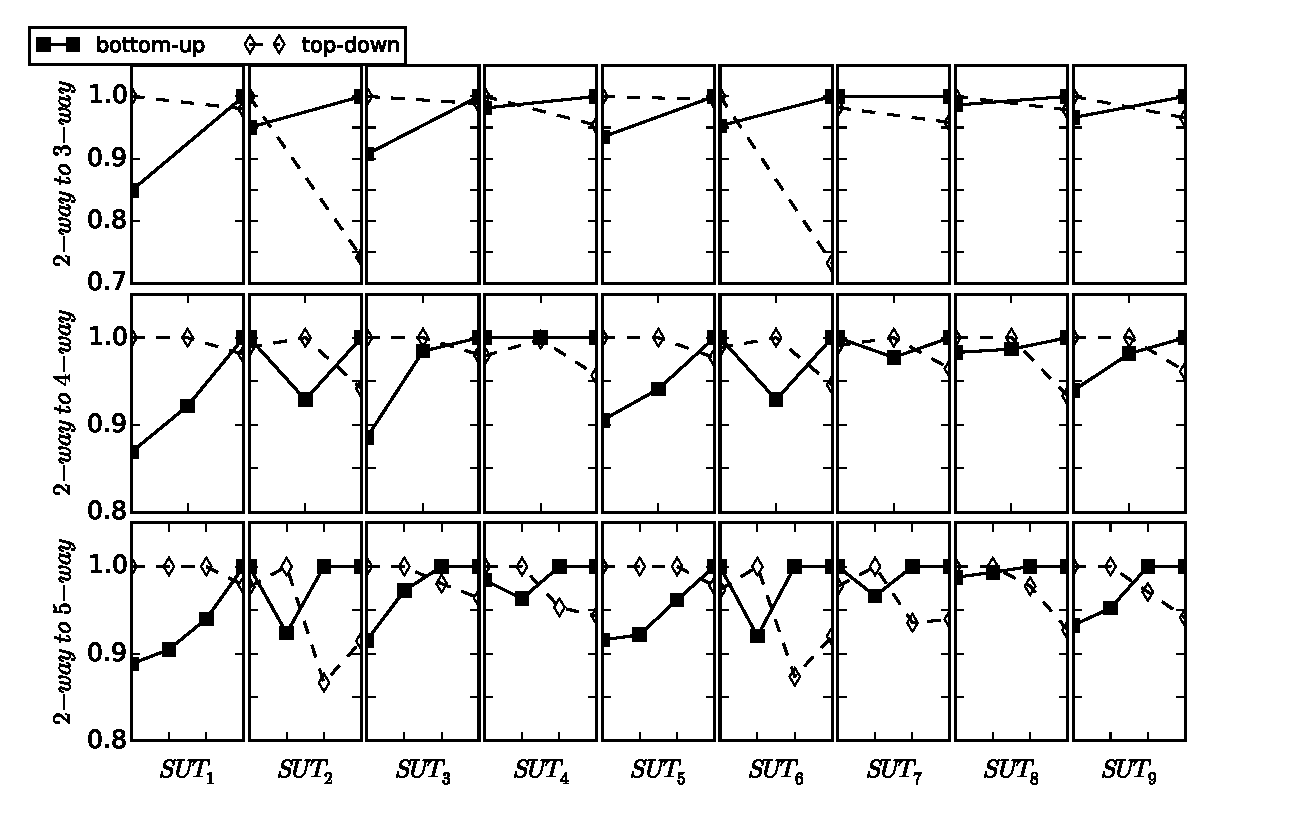
\includegraphics[width=6.0in]{experiment.eps}
\caption{The comparison of the two strategies}
\label{experiement}
\end{figure*}


In Fig.\ref{experiement}, there are three main rows, representing the results of three incremental covering arrays , $ICA([N_{2},N_{3}]; [2, 3],$ $ k ,v)$, $ICA$ $([N_{2},$ $N_{3}$ $,N_{4}];[2, 3,4], k ,v)$, and $ICA([N_{2},N_{3}$ $,N_{4},$ $N_{5}]$ $;[2,$ $ 3,4,5], k ,v)$, respectively.  The nine columns represents the nine SUTs in Table \ref{model_of_sut_of_subjects}. For each sub-figure in Fig.\ref{experiement}, the horizontal axis depicts the results of covering arrays of different strengths, and the vertical axis represents the size of the covering array. Note that we do not directly show the value of the size; instead, we normalize them so that they can be put into one figure. In detail, for each covering array of a subject, the point in the figure for one strategy indicates the proportion of the average size obtained by this strategy and the larger one of the two strategies.
% we put the into the figure, such that .
%
%This is because, the gap between the size of different-way covering array is too big to put into one figure.

From Fig.\ref{experiement}, we can observe that, for most cases, the \emph{top-down} strategy obtained smaller higher-strength covering arrays (about 90 \% of that of \emph{bottom-up}), while the \emph{bottom-up} strategy performed better at the lower-strength covering arrays. This conclusion coincides with the case study presented in Section 3.  There are also some exceptions; for example in the second row in Fig. \ref{experiement} ($ICA([N_{2},N_{3},N_{4}]; [2, 4], k ,v)$), the \emph{top-down} strategy generated smaller 2-way covering arrays for $SUT_{2}$, $SUT_{4}$, and $SUT_{6}$ than that of \emph{bottom-up}. One possible explanation for the exception is that the covering array generated by greedy approach AETG sometimes may produce more test cases than needed.


Above all, the preliminary results suggested that when the coverage strength of the final covering array is low, the \emph{bottom-up} strategy is preferred; otherwise, the \emph{top-down} strategy is a better choice.

Besides this, it is noted that the \emph{top down} strategy may generate larger lower strength arrays which are definitely to be executed while the \emph{bottom up} strategy may generate larger higher strength arrays which may not be executed. This usually happens when the current software under testing is expired for the releasing of the next version. In that case, the \emph{bottom-up} strategy is recommended.




%\begin{table}
%\caption{The incremental covering array to be constructed}
%\label{ica_to_constuct}
%\center
%\setlength{\tabcolsep}{3pt}
%\begin{tabular}{c | c | c }
%\hline  $ICA^{1}$:ICA((2,4),$10^{30}$)& $ICA^{2}$:ICA((2,4),$2^{100}$)& $ICA^{3}$:ICA((2,4),$10^{20}$) \\
%\hline  $ICA^{4}$:ICA((2,4),$7^{6}6^{7}5^{6}$) & $ICA^{5}$:ICA((2,4),$3^{13}$) & $ICA^{6}$:ICA((2,4),$8^{40}$ ) \\
%\hline  $ICA^{7}$:ICA((2,4),$15^{9}10^{6}$) & $ICA^{8}$:ICA((2,4),$4^{10}$) & $ICA^{9}$:ICA((2,4),$8^{20}$ ) \\
%\hline  $ICA^{10}$:ICA((2,4),$6^{10}$) & $ICA^{11}$:ICA((2,4),$4^{20}$) & $ICA^{12}$:ICA((2,4),$6^{20}$)\\\hline
%\end{tabular}
%  \end{table}
\section{Threats to Validity}
In this section, we will co

\section{Related work}

Combinatorial testing has been proven to a effective testing technique in practice \cite{kuhn2010practical}, especially on domains like configuration testing \cite{yilmaz2006covering,cohen2006testing,qu2008configuration} and software inputs testing \cite{cohen1997aetg,borazjany2012combinatorial,ghandehari2013applying}. The most important task in CT is to generate covering arrays, which support the checking of various valid interactions of factors that influence the system under testing.

Nie et al. \cite{nie2011survey} gave a survey for combinatorial testing, in which the methods for generating covering
arrays are classified. However, traditional static covering arrays can be hardly directly applied in practice, hence many adaptive methods are proposed.

Cohen et al. \cite{cohen2007exploiting,cohen2008constructing} studied the constraints that can render some test cases in the covering array invalid. They proposed a SAT-based approach to avoid the impact.
%Further, Ylimaz  \cite{dumlu2011feedback,yilmaz2013reducing} proposed a feed-back approach which can support dynamically detect and identify the unknown constraints, i.e., \emph{masking effects}. This approach can help to avoid the constraints in the latter generated test cases.
Nie et al.\cite{nie2013adaptive} proposed a model for adaptive CT, in which both the failure-inducing interactions and constraints can be dynamically detected and removed in the early test cases generation iteration. Further, the coverage strength of covering array can be adaptively changed as required. S.Fouch{\'e}  et al. \cite{fouche2009incremental} proposed the incremental covering array, and gave a method to generate it. The method can be deemed as a special case of \emph{bottom-up} strategy, with the only difference being that it used multiple lower-strength covering arrays instead only one in this paper to construct the higher-strength covering array. This is because their work needs to characterize the failure-inducing interactions in the covering array, in which ,multiple covering arrays can support a better diagnosis.

Calvagna et al. \cite{calvagna2013incrementally} proposed another work
%
%it hence use the classification tree method to classify the failure-inducing interaction, such that it should need to run multiple test cases, which is an augment of the bottom-up.


\section{Conclusions and future works}
This paper proposed two strategies for generating incremental covering arrays. Experimental results show that both strategies have their own advantages; \emph{top-down} strategy is better at generating higher-strength covering arrays, while \emph{bottom up} strategy performs better at lower-strength ones .

As a future work, we will apply more covering array generation algorithms, to compare their performance at generating incremental covering arrays. Another interesting work is to combine the two strategies, so that we can first select a median coverage strength \emph{t} and generate incremental covering arrays by \emph{top-down} strategy. Then if the maximal-way covering array is generated, we can use \emph{bottom-up} strategy to generate further higher-strength covering arrays. We believe such a combination strategy may offer a better performance.
% An example of a floating figure using the graphicx package.
% Note that \label must occur AFTER (or within) \caption.
% For figures, \caption should occur after the \includegraphics.
% Note that IEEEtran v1.7 and later has special internal code that
% is designed to preserve the operation of \label within \caption
% even when the captionsoff option is in effect. However, because
% of issues like this, it may be the safest practice to put all your
% \label just after \caption rather than within \caption{}.
%
% Reminder: the "draftcls" or "draftclsnofoot", not "draft", class
% option should be used if it is desired that the figures are to be
% displayed while in draft mode.
%
%\begin{figure}[!t]
%\centering
%\includegraphics[width=2.5in]{myfigure}
% where an .eps filename suffix will be assumed under latex,
% and a .pdf suffix will be assumed for pdflatex; or what has been declared
% via \DeclareGraphicsExtensions.
%\caption{Simulation Results}
%\label{fig_sim}
%\end{figure}

% Note that IEEE typically puts floats only at the top, even when this
% results in a large percentage of a column being occupied by floats.


% An example of a double column floating figure using two subfigures.
% (The subfig.sty package must be loaded for this to work.)
% The subfigure \label commands are set within each subfloat command, the
% \label for the overall figure must come after \caption.
% \hfil must be used as a separator to get equal spacing.
% The subfigure.sty package works much the same way, except \subfigure is
% used instead of \subfloat.
%
%\begin{figure*}[!t]
%\centerline{\subfloat[Case I]\includegraphics[width=2.5in]{subfigcase1}%
%\label{fig_first_case}}
%\hfil
%\subfloat[Case II]{\includegraphics[width=2.5in]{subfigcase2}%
%\label{fig_second_case}}}
%\caption{Simulation results}
%\label{fig_sim}
%\end{figure*}
%
% Note that often IEEE papers with subfigures do not employ subfigure
% captions (using the optional argument to \subfloat), but instead will
% reference/describe all of them (a), (b), etc., within the main caption.


% An example of a floating table. Note that, for IEEE style tables, the
% \caption command should come BEFORE the table. Table text will default to
% \footnotesize as IEEE normally uses this smaller font for tables.
% The \label must come after \caption as always.
%
%\begin{table}[!t]
%% increase table row spacing, adjust to taste
%\renewcommand{\arraystretch}{1.3}
% if using array.sty, it might be a good idea to tweak the value of
% \extrarowheight as needed to properly center the text within the cells
%\caption{An Example of a Table}
%\label{table_example}
%\centering
%% Some packages, such as MDW tools, offer better commands for making tables
%% than the plain LaTeX2e tabular which is used here.
%\begin{tabular}{|c||c|}
%\hline
%One & Two\\
%\hline
%Three & Four\\
%\hline
%\end{tabular}
%\end{table}


% Note that IEEE does not put floats in the very first column - or typically
% anywhere on the first page for that matter. Also, in-text middle ("here")
% positioning is not used. Most IEEE journals/conferences use top floats
% exclusively. Note that, LaTeX2e, unlike IEEE journals/conferences, places
% footnotes above bottom floats. This can be corrected via the \fnbelowfloat
% command of the stfloats package.



% conference papers do not normally have an appendix


% use section* for acknowledgement
\section*{Acknowledgment}
This work was supported by the National Natural Science Foundation of China (No. 61272079), the Research Fund for the Doctoral Program of Higher Education of China (No.20130091110032), the Science Fund for Creative Research Groups of the National Natural Science Foundation of China(No. 61321491), and the Major Program of National Natural Science Foundation of China (No. 91318301)




% trigger a \newpage just before the given reference
% number - used to balance the columns on the last page
% adjust value as needed - may need to be readjusted if
% the document is modified later
%\IEEEtriggeratref{8}
% The "triggered" command can be changed if desired:
%\IEEEtriggercmd{\enlargethispage{-5in}}

% references section

% can use a bibliography generated by BibTeX as a .bbl file
% BibTeX documentation can be easily obtained at:
% http://www.ctan.org/tex-archive/biblio/bibtex/contrib/doc/
% The IEEEtran BibTeX style support page is at:
% http://www.michaelshell.org/tex/ieeetran/bibtex/
\bibliographystyle{IEEEtran}
% argument is your BibTeX string definitions and bibliography database(s)
\bibliography{incremental}
%
% <OR> manually copy in the resultant .bbl file
% set second argument of \begin to the number of references
% (used to reserve space for the reference number labels box)
%\begin{thebibliography}{1}
%
%\bibitem{IEEEhowto:kopka}
%H.~Kopka and P.~W. Daly, \emph{A Guide to \LaTeX}, 3rd~ed.\hskip 1em plus
%  0.5em minus 0.4em\relax Harlow, England: Addison-Wesley, 1999.
%
%\end{thebibliography}




% that's all folks
\end{document}


